\begin{tikzpicture}[
  x=1cm,
  y=1cm,
  >=Latex,
  arrow/.style={->, very thick, draw=black!65},
  rewardarrow/.style={->, thick, draw=red!70!black},
  card/.style={draw=black!18, fill=white, rounded corners=2pt, minimum width=4.25cm, minimum height=3.55cm, inner sep=6pt},
  smallbox/.style={draw=red!65!black, fill=red!8, rounded corners=2pt, minimum width=2.48cm, minimum height=0.46cm, align=center},
  every node/.style={font=\sffamily\small}
]
  % Column headings
  \node[font=\sffamily\Large] at (0,3.78) {Prompt};
  \node[font=\sffamily\Large] at (5.50,3.78) {MedGemma};
  \node[font=\sffamily\Large] at (11.00,3.78) {Completions};
  \node[font=\sffamily\Large] at (15.75,3.78) {Reward};

  % Prompt card
  \node[card] (prompt-card) at (0,1.68) {};
  \node[inner sep=0pt] (ct) at (-1.15,1.92)
    {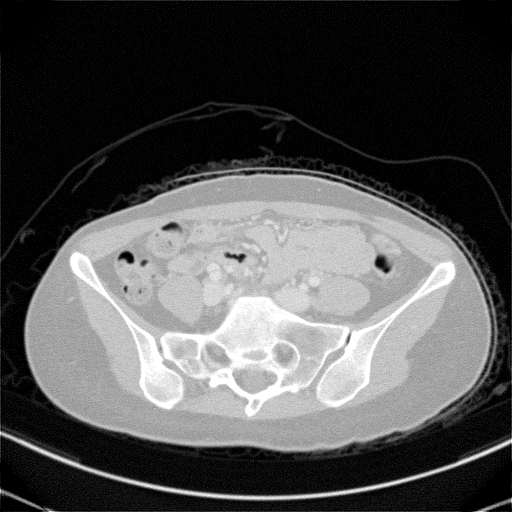
\includegraphics[width=1.15cm,height=1.15cm]{figures/ldct_example.png}};
  \node[font=\sffamily\scriptsize] at (-1.15,1.12) {LDCT image};
  \node[align=left, text width=1.86cm] at (0.95,1.95)
    {User:\\\textbf{Predict MOS score.}};
  \draw[black!50, line width=0.8pt] (-1.58,0.78) -- (1.58,0.78);
  \draw[black!50, line width=0.8pt] (-1.58,0.57) -- (1.10,0.57);
  \node[align=center, font=\sffamily\scriptsize, text width=3.35cm] at (0,0.28)
    {prompt-only image chat};

  % MedGemma-inspired medical AI icon and LoRA adapter
  \node[draw=orange!75!black, fill=orange!8, rounded corners=3pt, minimum width=3.18cm, minimum height=3.25cm] (model) at (5.50,1.80) {};
  \begin{scope}[shift={(5.50,2.28)}]
    \fill[blue!70!black] (-0.62,0.28) circle (0.34);
    \fill[blue!70!black] (-0.88,-0.10) circle (0.34);
    \fill[blue!70!black] (-0.48,-0.34) circle (0.34);
    \fill[cyan!70!green] (0.62,0.28) circle (0.34);
    \fill[cyan!70!green] (0.88,-0.10) circle (0.34);
    \fill[cyan!70!green] (0.48,-0.34) circle (0.34);
    \fill[blue!60!black] (-0.18,-0.42) rectangle (0.00,0.54);
    \fill[cyan!65!green] (0.00,-0.42) rectangle (0.18,0.54);
    \draw[white, line width=1.3pt] (-0.34,0.00) -- (0.34,0.00);
    \draw[white, line width=1.3pt] (0,-0.30) -- (0,0.32);
    \draw[black!55, line width=0.45pt] (-0.78,0.18) -- (-0.42,0.18) -- (-0.18,0.36);
    \draw[black!55, line width=0.45pt] (-0.76,-0.10) -- (-0.38,-0.10) -- (-0.14,-0.22);
    \draw[black!55, line width=0.45pt] (0.78,0.18) -- (0.42,0.18) -- (0.18,0.36);
    \draw[black!55, line width=0.45pt] (0.76,-0.10) -- (0.38,-0.10) -- (0.14,-0.22);
    \foreach \p in {(-0.82,0.18),(-0.76,-0.10),(0.82,0.18),(0.76,-0.10)} {
      \fill[white] \p circle (0.045);
      \draw[black!55] \p circle (0.045);
    }
    \draw[blue!70!black, line width=1.1pt] (-0.54,-0.78) .. controls (-0.05,-0.36) and (0.22,-1.02) .. (-0.32,-1.34);
    \draw[cyan!70!green, line width=1.1pt] (0.54,-0.78) .. controls (0.05,-0.36) and (-0.22,-1.02) .. (0.32,-1.34);
    \draw[black!35, line width=0.35pt] (-0.15,-0.98) -- (0.15,-0.84);
    \draw[black!35, line width=0.35pt] (-0.12,-1.18) -- (0.12,-1.04);
  \end{scope}
  \node[align=center, font=\sffamily\bfseries\small, text=cyan!45!black] at (5.50,0.55) {MedGemma 1.5};
  \node[draw=green!55!black, fill=green!10, rounded corners=2pt, minimum width=1.75cm, minimum height=0.48cm, align=center] (lora) at (5.50,-0.50)
    {LoRA};
  \draw[arrow] (lora.north) -- (model.south);
  \node[font=\sffamily\scriptsize, align=center] at (5.50,-1.10) {base or SFT\\initialization};

  % Completion card
  \node[card] (completion-card) at (11.00,1.68) {};
  \node[align=center, text width=3.35cm] at (11.00,2.82) {Sampled completions};
  \node[smallbox] (c1) at (11.00,2.32) {\texttt{\{"rating": 2.0\}}};
  \node[smallbox] (c2) at (11.00,1.78) {\texttt{\{"rating": 2.5\}}};
  \node[smallbox] (c3) at (11.00,1.24) {\texttt{\{"rating": 3.0\}}};
  \node[smallbox] (c4) at (11.00,0.70) {\texttt{\{"rating": 4.0\}}};
  \node[align=center, font=\sffamily\scriptsize, text width=3.15cm] at (11.00,0.16)
    {candidate group};

  % Reward card
  \node[card, minimum width=3.55cm] (reward-card) at (15.75,1.68) {};
  \node[align=center, text width=3.10cm] at (15.75,2.76) {Parse and score};
  \node[draw=blue!65!black, fill=blue!7, rounded corners=2pt, minimum width=2.68cm, minimum height=0.58cm, align=center] (mos) at (15.75,2.04)
    {Reference MOS $y$};
  \node[draw=red!65!black, fill=red!8, rounded corners=2pt, minimum width=2.88cm, minimum height=0.72cm, align=center] (reward) at (15.75,1.08)
    {$R(\hat{y},y)=-|\hat{y}-y|$};
  \node[align=center, font=\sffamily\scriptsize, text width=3.10cm] at (15.75,0.30)
    {higher reward for closer MOS};

  % Forward and reward flow
  \draw[arrow] (prompt-card.east |- model.west) -- (model.west);
  \draw[arrow] (model.east) -- (completion-card.west |- model.east);
  \draw[arrow] (completion-card.east |- reward.west) -- (reward.west);
  \node[font=\sffamily\scriptsize, align=center] at (2.75,2.25) {image +\\instruction};
  \node[font=\sffamily\scriptsize, align=center] at (8.10,2.28) {sampled\\MOS texts};
  \node[font=\sffamily\scriptsize, align=center] at (13.55,1.48) {parsed\\scores};
  \draw[rewardarrow] (reward.east) -- ++(0.48,0) |- (lora.east);
  \node[font=\sffamily\scriptsize, text=red!70!black, align=center, fill=white, inner sep=1pt] at (10.20,-0.96) {GRPO reward\\update};
\end{tikzpicture}
